\chapter{Introduction}

An organism's capabilities are encoded by the sequence of nucleotides found within its DNA \cite{crick1970central}. DNA sequencing \footnote{Genome sequencing involves taking multiple copies of an organism's genome, fragmenting them randomly, and placing them into a sequencing machine \cite{shendure2017dna}. This machine reads the sequence of nucleotides of each fragment  \cite{shendure2017dna}. These potentially overlapping fragments are sequenced in parallel for higher throughput. After sequencing, the order of nucleotides of these fragment are the used, \textit{in silico}, to assemble a read out of the organism's entire genome sequence \cite{wajid2012review}. The assembly process involves stitching together overlapping fragments with highly similar head and tail sequences, which is analogous to putting together pieces of a puzzle \cite{wajid2012review}.} allows us to read these sequences and, through software, learn more about an organism's potential capabilities without having to study it \textit{in vivo} \cite{de2012bioinformatic}. In an environmental microbiology context such sequenced genomes are used is learn more about microorganisms' metabolic capabilities and possibly shed light on their ecological role \cite{de2012bioinformatic}. In an applied context, predictions of such metabolic capabilities are also useful. Certain microbes are more suitable for specific bioprocesses \footnote{A bioprocess is a process carried out by living cells or their components. They are used across a verity of industrial sectors including energy \cite{deublein2011biogas}, mining \cite{dew1997biox}, manufacturing \cite{thodey2014microbial} and environmental remediation \cite{alexander1999biodegradation}.} and this suitability is based on their metabolic capabilities. The metabolisms of the organisms involved influence the process's conditions and overall efficiently \cite{doran1995bioprocess,liu2016bioprocess}. In both applied and environmental contexts, genomically derived genome-scale metabolic reconstruction models can be used to simulate nutrients flow through and between organisms \cite{magnusdottir2017generation, arkin2018kbase, faria2018improving}. In a genetic engineering context, genomically derived information about organism can be used to select what traits to remove from organisms or move between them \cite{strohl2001biochemical}.

Advances in DNA sequencing technology over the past decade have revolutionized our ability to acquire bacterial and archaeal genomes. For example, with newer sequencing technologies such as Oxford Nanopore \cite{jain2016oxford}, a bacterial genome can be acquired in a matter hours \cite{Lu2016,Cao2017}. Researchers have now moved on to extracting the genomes of unculturable microorganisms from environmental samples using culture-free techniques such a metagenomic \cite{quince2017shotgun} and single cell \cite{gawad2016single} sequencing. Over the past few years, the tree of life has been significantly expanded by the Metagenome Assembled Genomes (MAGs) \footnote{Metagenomic sequencing involves sequencing the genomes a mixture of organisms in parallel \cite{quince2017shotgun}. The resulting sequenced fragments are not labelled as to which organisms they came from. In software, genome assembly and an additional process called genome binning are used to generate multiple genomes out a the pool of sequenced fragments generated by the sequencer \cite{quince2017shotgun, sangwan2016recovering}. These separated genomes are called Metagenome Assembled Genomes (MAGs) if they are of high completeness and low in contamination \cite{sangwan2016recovering}. \label{metagenomics-footnote}} of these unculturable organisms \cite{Hug2016,Parks2017}. With microbiologists ability to gather new genomes rectified, the problem now shifts to interpreting this new wealth of genomic data. 

Due to their vast size and information density, interpretation of genomes is often assisted by software. The software platform presented in this thesis, Micromeda, is such a software tool. It streamlines the prediction of an organism's metabolic capabilities and, through a web-based data visualization interface, assists users in comparing the metabolisms of multiple organisms found within an environment. Pygenprop, a library built to assist in the development of Micromeda, allows users to perform such comparisons programmatically. A key feature of both Micromeda and Pygenprop is their ability to not only compare the predicted metabolic features of organisms, in terms of biochemical pathways present, but also allow users to access the underlying protein sequences that support these predictions. Details about the information presented by Micromeda, the database it uses and its expected use cases are presented within this chapter. The following chapters will discuss Pygenprop and Micromeda's implementation.

\section{Enzymes and Biochemical Pathways}

For many systems, both environmental and industrial processes can be carried out biochemically. From a biological context, such processes are carried out via a series of chemical reactions catalysed by biological enzymes. Enzymes act as biological catalysts that accelerate chemical reactions via the lowering their required activation energy \cite{segel1975enzyme}. The majority of enzymes are made from protein \cite{kruger1982self}. According to the central dogma of molecular biology, all proteins, whether structural or enzymatic, within cells are encoded for by genes that are a subset of an organism's DNA-based genome \cite{crick1970central}. Within prokaryotic \footnote{Bacteria and Archaea form two distinct branches on the tree of live. The cells of these prokaryotic organisms generally \cite{nevo2007thylakoid,cameron2013biogenesis,bazylinski2004magnetosome,van2008combined,adams2000heterocyst,o2000biofilm} lack membrane bound cellular compartments (organelles) and are unicellular. The rest of the tree of life is made up of eukaryotes that are have such organelles and can be multicellular \cite{baldauf2003deep}. Plants, animals and fungi are eukaryotes.} organisms such as Archaea and Bacteria, most often one gene maps to one protein, or protein subunit, produced. When an enzyme is required by a cell, the DNA gene providing a blueprint for it is transcribed to RNA transcripts \cite{crick1970central}. These transcripts later provide instructions to a ribosome on how to join a series of ammo acid residues together into a specific polypeptide biopolymer \cite{crick1970central}. This biopolymer then spontaneously folds, based of chemical properties of its individual amino acid residues, into a unique three dimensional shape that forms an enzymatic protein \cite{fersht1992folding}. The order of the residues in the polypeptide that forms a protein is encoded for by its DNA gene and is crucial to an enzyme's folded shape and activity towards different chemical reactions. This order is called a sequence and is also crucial for determining what chemical compounds, called substrates, are most likely to be used as inputs into a reaction catalysed by an enzyme \cite{fersht1992folding,fersht1999structure}. Mutations in the gene's sequence can cause changes in substrate specificity (i.e., what compounds are most likely for an enzyme to use as inputs into a reaction). The genes that encode for enzymes are often under selective pressure (i.e., organisms with with more efficient enzymes may produce more offspring) and thus evolve over time \cite{zhang2003evolution,whelan2001general}. Often genes are duplicated and duplicates are free to evolve to tackle new substrates \cite{zhang2003evolution}. All genes are derived from the duplication and mutation of other genes and thus all enzymes are related to all other enzymes \cite{zhang2003evolution,whelan2001general}. Thus, enzyme's that facilitate similar chemical reactions often \cite{galperin1998analogous} have similar sequences of amino acid residues, structures and genes that encode them \cite{zhang2003evolution}.

A biochemical pathway represents a series of chemical reactions, that when chained together, are beneficial to a cell \cite{michal2012biochemical}. For example, the breaking down of a nutrient macromolecule into pieces that cells can use or the build up of components of cellular structure \cite{wagner2012metabolic}. Each reaction step in a pathway is often \cite{keller2015widespread,tawfik2010enzyme} catalysed by a specific enzyme whose amino acid sequence, and thus structure and activity, is optimized for the particular reaction \cite{michal2012biochemical,zhang2003evolution,fersht1999structure}. Thus, there is a mapping between specific enzymes (and the genes encoding them) and chemical reaction steps in biochemical pathways \cite{thiele2010protocol}. As a result, by reading the genome, researchers can predict what biochemical pathways an organism may possess \cite{abubucker2012metabolic,thiele2010protocol}. Genes encoding for enzymes that all assist in the same biochemical pathway are often co-located spatially on a host's genome \cite{lawrence1999selfish,de2010genomic}. Sometimes these genes are transcribed together before translation into individual proteins \cite{blumenthal1998gene,danchin1980coordinate}. Due to the evolution of genes and enzymes over time, biochemical pathways can also change over time \cite{hochachka2002biochemical,raymond2006effect}. New enzymes or derivatives of existing enzymes can replace those enzymes that catalysed pathway steps in the past \cite{jensen1976enzyme}. This swapping also follows evolutionary patterns \cite{morowitz1999theory, raymond2006effect,wagner2012metabolic}. Organisms from different environments may have different enzymes that catalyse pathway reactions in a different way \cite{raymond2006effect}. Often chemical compounds produced half way through a pathway can be used as inputs for an entirely different pathway \cite{wagner2012metabolic,stelling2002metabolic}. In addition, the output from one pathway, for example monomers from the break down of a macro-nutrient, may be the input for a second biochemical pathways that builds cellular structures \cite{wagner2012metabolic,stelling2002metabolic}. Thus, as all pathways in a cell are somehow connected, the pathways in a cell form a network of reactions \cite{wagner2012metabolic,stelling2002metabolic}. This network forms the cell's metabolism and is called its metabolic network \cite{wagner2012metabolic}.

\section{Pathway Databases}

For many decades scientists have been designing and executing studies to figure out what individual enzymes do and what substrates they can catalyse. They have also found what what genes encode for these enzymes. The results of such studies are published in literature and databases have been compiled that store the results of these studies. Specifically, what genes encode for what enzymes, what enzymes catalyse what reactions, and what reactions belong to what biochemical pathways. These databases also map how pathways are connected to each other within cells' metabolic networks. Examples of such databases include KEGG \cite{kanehisa2000kegg}, MetaCyc \cite{karp2002metacyc}, Genome Properties \cite{richardson2018genome}, SEED subsystems \cite{overbeek2005subsystems}, Reactome \cite{croft2013reactome}, and many others. Such databases are often optimized to contain data about a specific organism (e.g. humans \cite{croft2013reactome}), clade on the tree of life (e.g. prokaryotes \cite{richardson2018genome}) or area of metabolism (e.g. small molecule production \cite{Jewison2014}).

\section{The State of Pathway Analysis}

As the breadth of the information within pathway databases increases, it is increasingly being used for the automation of pathway analysis. Researchers are automating their work flows by developing software tools that help them predict the presence of pathways in novel organisms or build models that predict nutrient flux through cells. Such tools are often released in the form of software toolchains (i.e. pipelines) where each step is performed by a separate bioinformatics application. Such pipelines take an organism's DNA genome sequence, performs \textit{in-silico} transcription and translation (Fig. \ref{fig:pathway-analysis-steps}), identifies enzymes and figures out what pathways they belong to via information contained within pathway databases (Fig. \ref{fig:pathway-analysis-overview}). These tools perform some or all of the following key steps.

\begin{enumerate}
\item Prediction of what genes are present in an organism's genome.
\item Translation of these genes' sequences to protein for reduced redundancy (Fig. \ref{fig:pathway-analysis-steps}). \footnote{There are four types of nucleotide monomers in the DNA biopolymer. Each is assigned a letter A,T, C or G. For protein coding genes, three letter codes (e.g. ATC, or CCG) in the DNA sequence, called codons, map to specific amino acids added to the translated protein sequence. Multiple types of three letter codes can cause the addition of a single amino acid type. Storing protein sequences instead of DNA sequences reduces redundancy in two ways. Firstly, by reducing the length of the information to be stored by one third due to a three to one letter mapping between DNA and protein sequences. Secondly, by replacing multiple sets of three DNA letters with a single amino acid letter due to codon to amino acid mappings. An added benefit is that translation of DNA sequences to protein masks mutations in a DNA sequence that do not change protein sequence and thus enzyme function.} 
\item Taking known enzymatic protein sequences from pathway databases and using them to search the above predicted proteins to find those with high sequence similarity. Predicted proteins with high sequence similarity to known enzymes are more likely to carry out the same enzymatic function. This process is called protein annotation (Fig. \ref{fig:pathway-analysis-steps}).
\item Using these newly found enzymes to figure out what chemical reactions could possibly be carried out by an organism.
\item Chaining these these reactions together to figure out what biochemical pathways are likely to be possessed by the organism (Fig. \ref{fig:pathway-analysis-steps}).
\item Presentation of information about the pathways present and enzymes found in a way that is comprehensible by users.
\end{enumerate}

\begin{figure}[!ht]
  \centering
	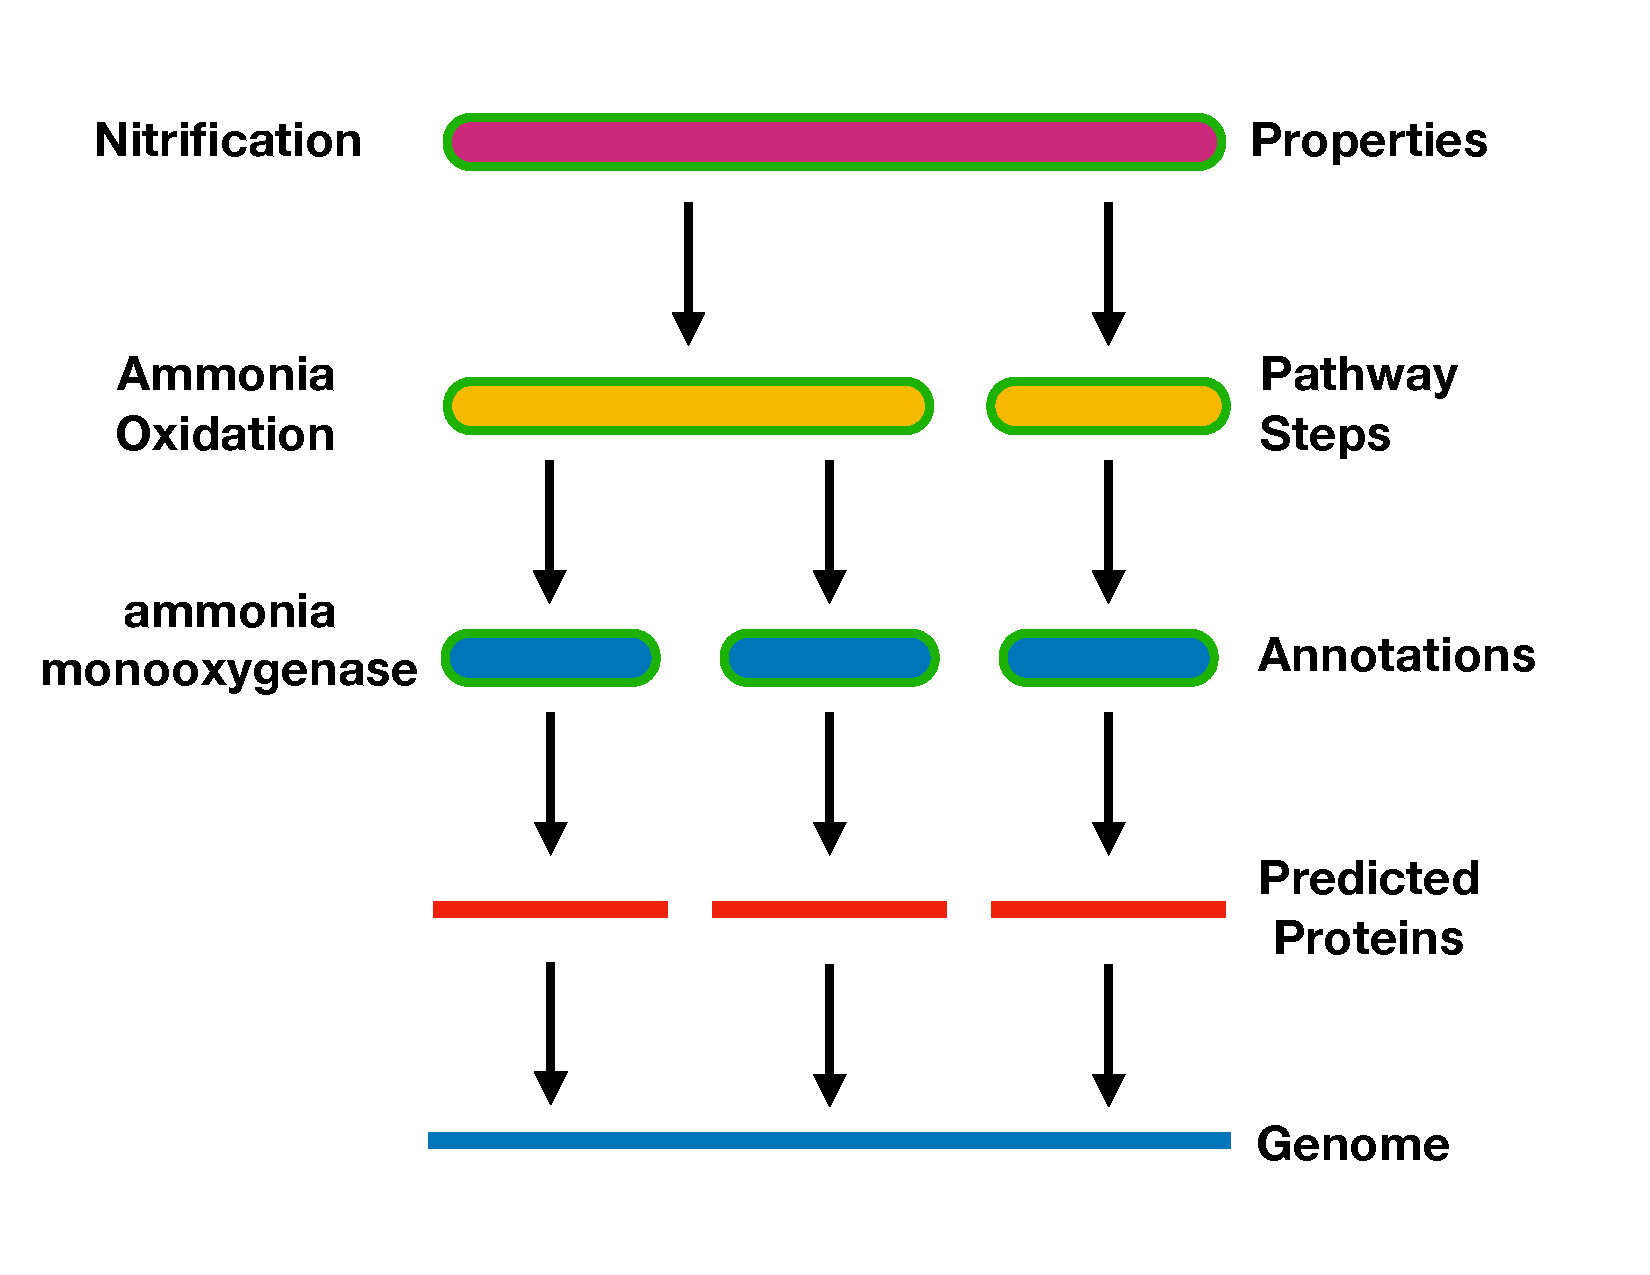
\includegraphics[width=0.8\textwidth]{media/pathway_analysis_steps.pdf}
	 \caption{Several several steps are required to go from an organism's genome sequence to a prediction of its metabolic capabilities.}
	 \label{fig:pathway-analysis-steps}
\end{figure}

\begin{figure}[!ht]
  \centering
	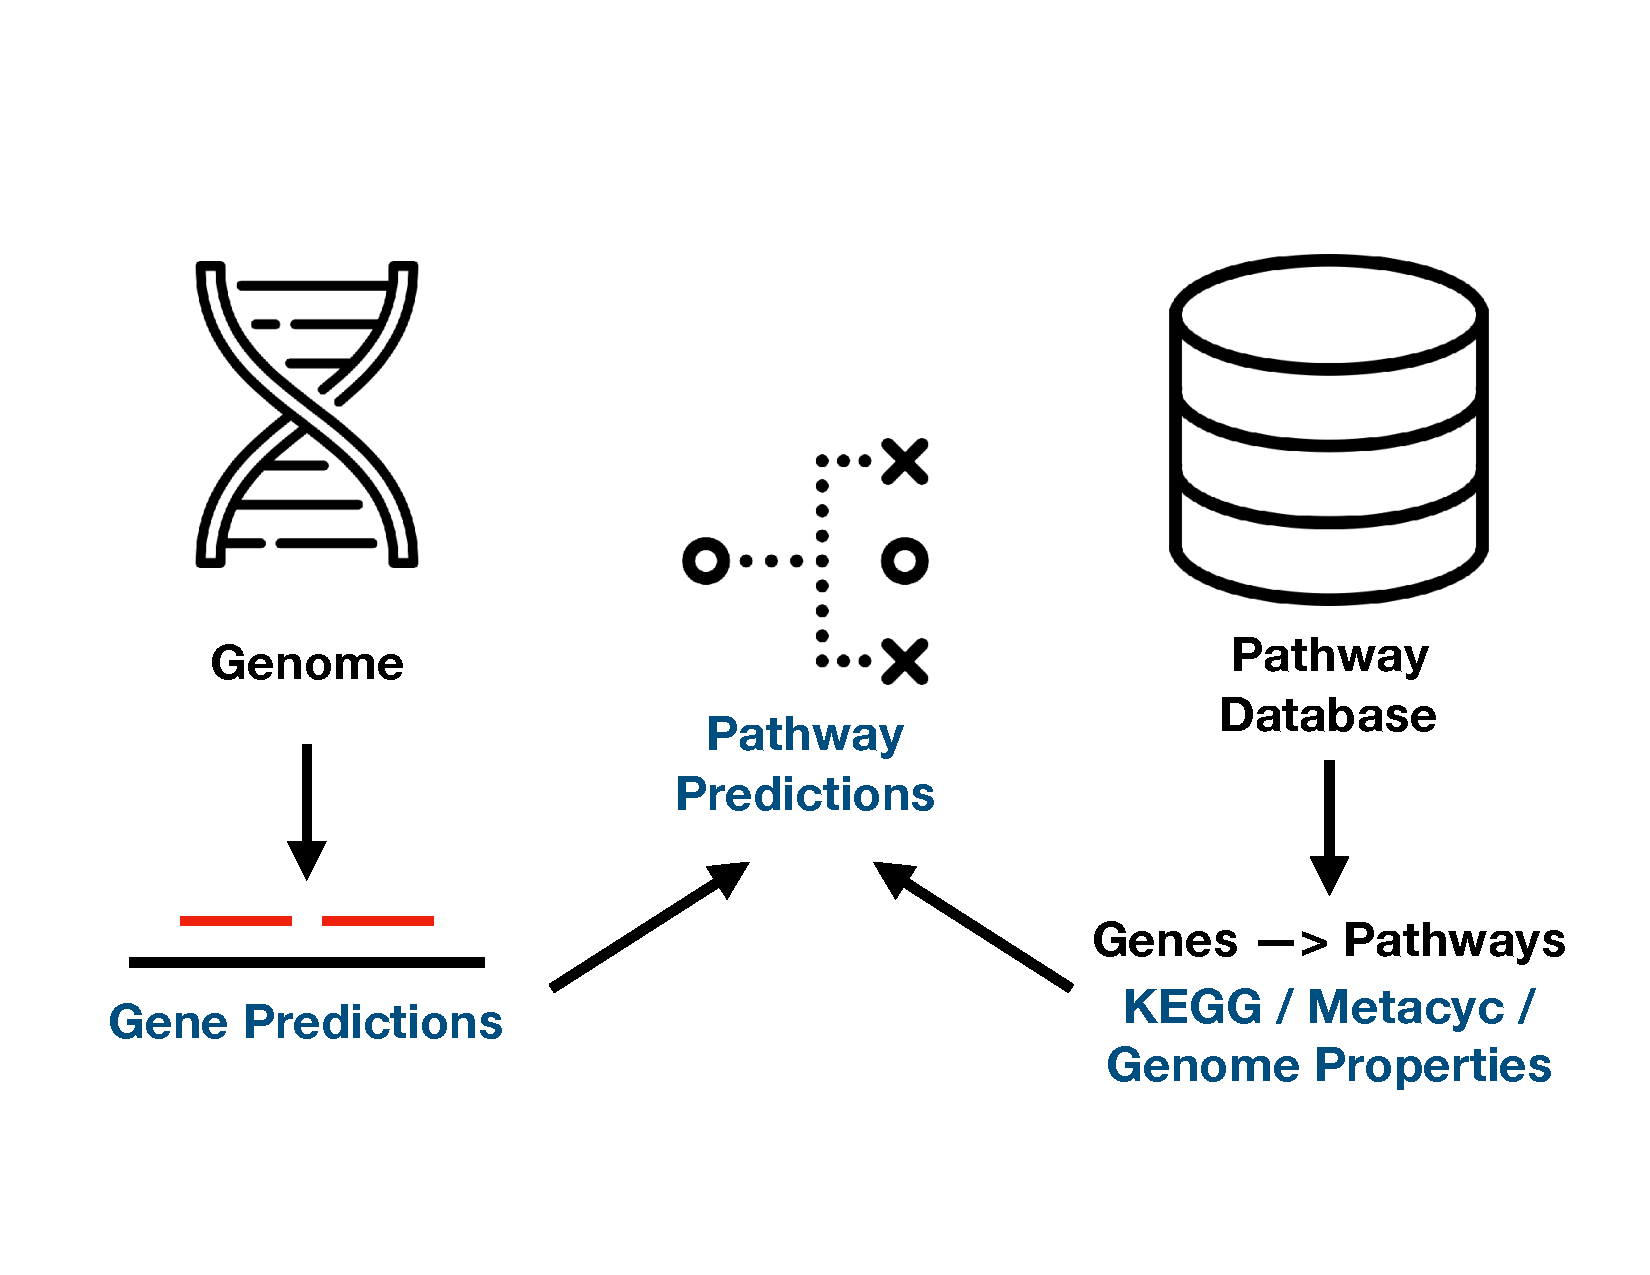
\includegraphics[width=0.8\textwidth]{media/pathway_bioinformatics.pdf}
	 \caption{Predicting the biochemical pathways that an organism may possess involves combining a predictions of what genes an organisms possesses with information about what genes are required by what pathways.}
	 \label{fig:pathway-analysis-overview}
\end{figure}

Some pipelines only work with pathway data from a specific database. For example, Pathway Tools can only present information about pathways found within the MetaCyc database. Often pipelines are optimized for generating data from the genomes of a specific clade on the tree of life. For example, Prokka, a pipeline that predicts genes and annotates protein sequences, is only designed to work with the genomes of prokaryotic organisms. Prokka only carries out the first few of the above list. Some tools can perform all the above steps. For example, the metagenomics pipeline Automatic Tool for Local Assembly Structures (ATLAS) can perform, in addition to generating genomes from raw sequencing reads, can perform pathway annotation on these genomes. ATLAS uses Prokka internally for some of its steps. Such bioinformatics pipelines can be deployed in two ways. They can either be installed on to a user's computer where genomes can be processed directly or they can deployed on to web server where users can upload their genomes for remote processing.

\section{The Current Bottlenecks of High Throughput Pathway Analysis}

Due to the current plethora of tools for genome annotation and pathway determination, figuring out what pathways are possessed by single organisms is becoming a solved problem. Researchers have moved on from analysing the pathways of a single organism to comparing the presence and absence of pathways across organisms. Such comparisons are in hope of finding information about these organism's ecological roles, evolution or suitability towards different industrial tasks. For example, the genomes of organisms that are closely related phylogenetically could be compared to determine those that may have lost or gained a pathway over time (Fig. \ref{fig:phylogenetic-comparison}). Alternatively, the pathways possessed by multiple organisms from within the same environment could be compared to shed light on their potential ecological niches (Fig. \ref{fig:metagenomics}). Pathway comparisons could also be used industrially to select organisms to add to co-cultures. For example, microbes that have fewer virulence associated pathways are more likely to act synergistic with the other organisms within a culture.

\begin{figure}[!ht]
  \centering
	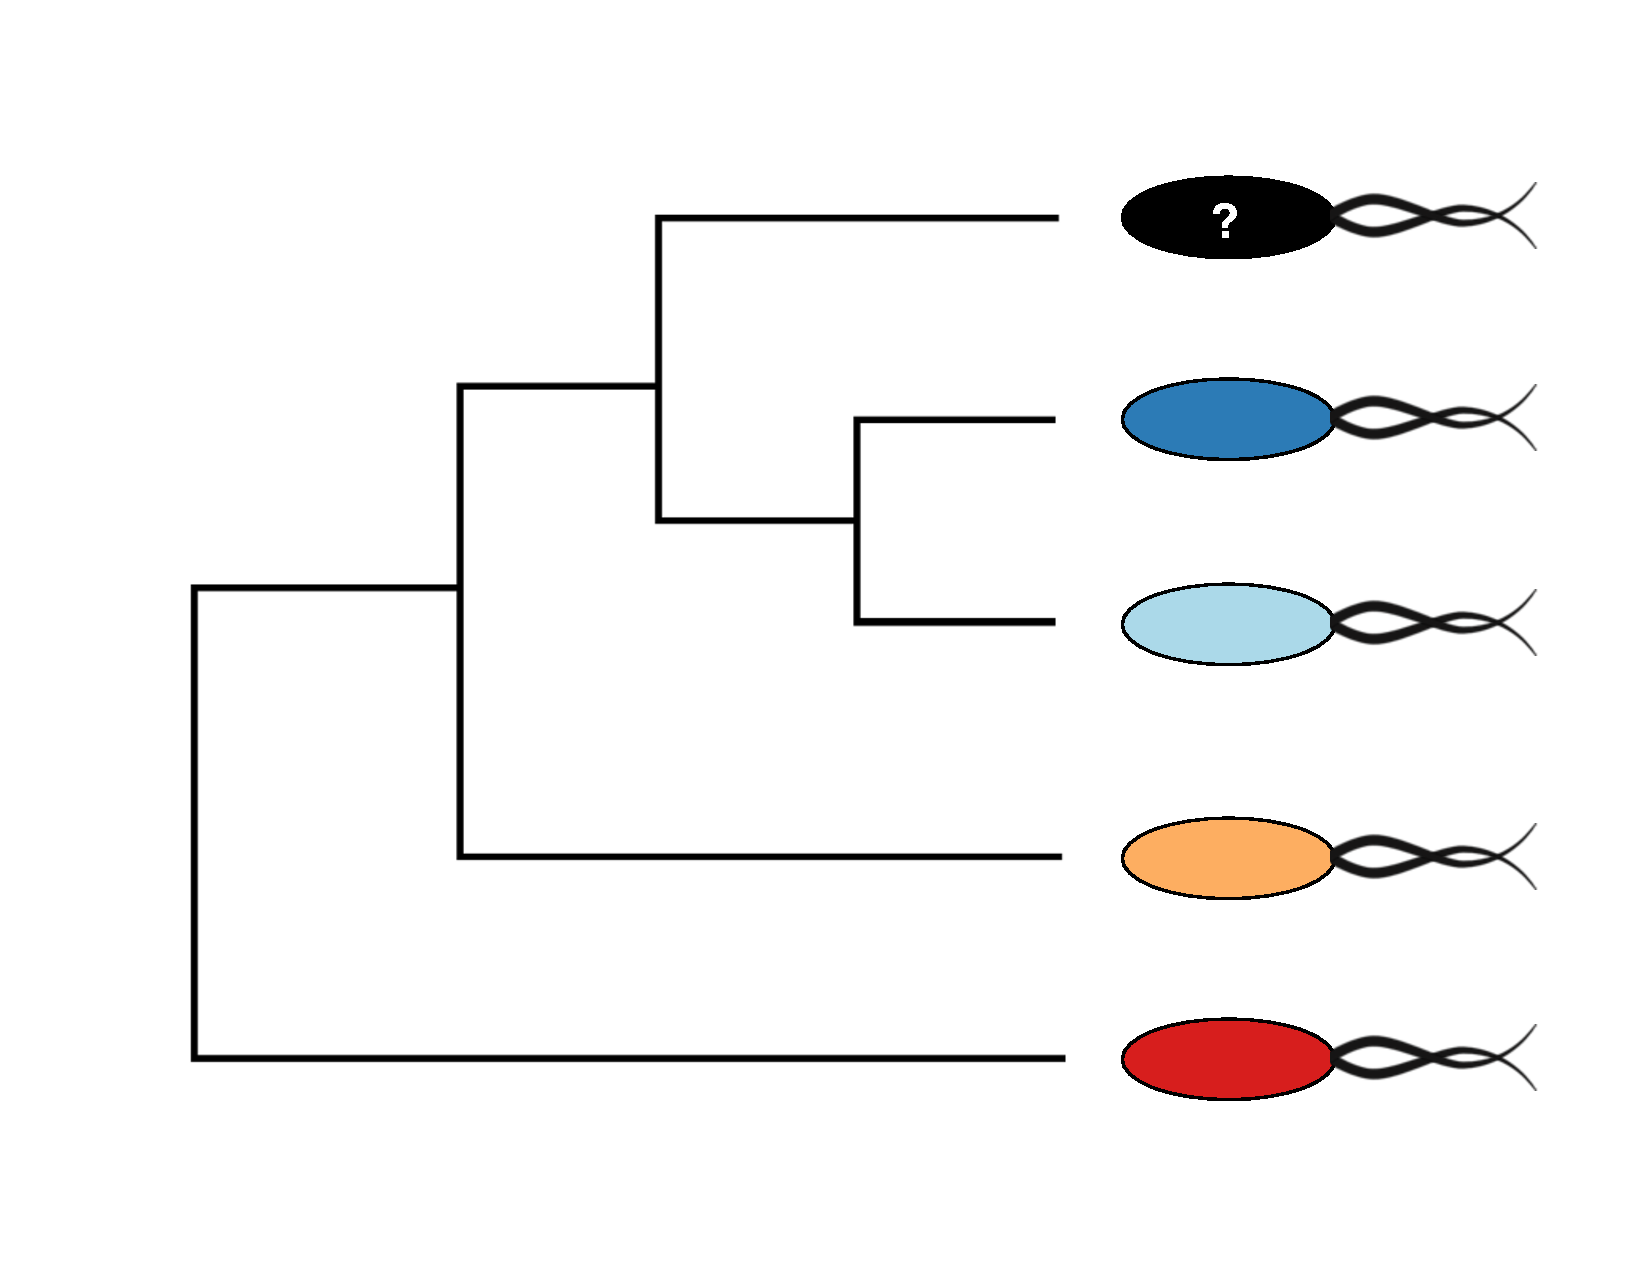
\includegraphics[width=0.7\textwidth]{media/compare-phylogenetically.pdf}
	 \caption{The pathways possessed by a novel organism (black) can be compared to those of closely related species.}
	 \label{fig:phylogenetic-comparison}
\end{figure}

\begin{figure}[!ht]
  \centering
	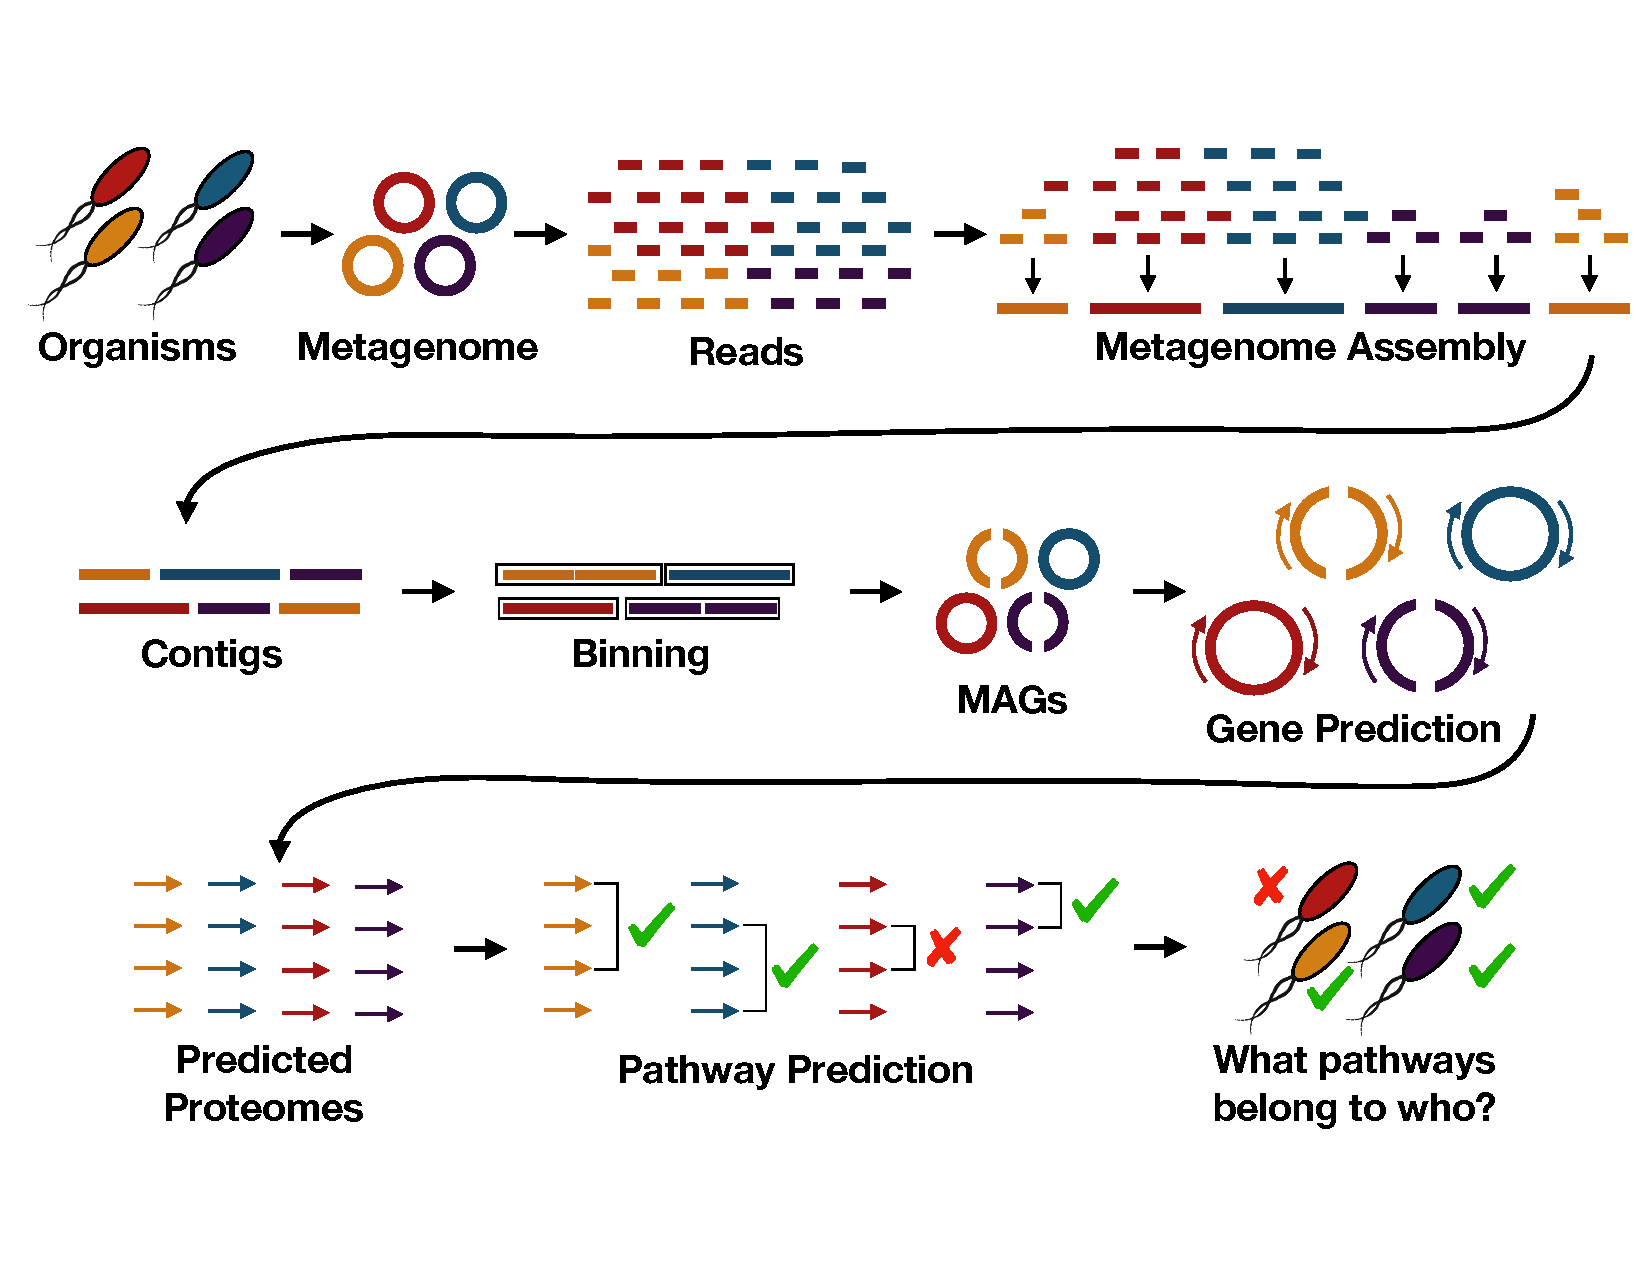
\includegraphics[width=0.7\textwidth]{media/metagenomics.pdf}
	 \caption{Metagenomics involves comparisons of multiple organism genomes found with the same environmental sample. As discussed in Footnote \ref{metagenomics-footnote}, bioinformatics techniques can be used to separate out individual genomes from a metagenomics samples. Pathway annotation can be performed on these genomes and used to compare the pathways possessed by different organisms from the same environment. Metagenomics bioinformatics pipelines such as Atlas can perform all the steps illustrated.}
	 \label{fig:metagenomics}
\end{figure}

Although assigning pathway presence and absence to individual organisms can be done quite rapidly, the comparison of these results across multiple organisms is currently a huge bottleneck. Often pathway annotation tools that can process multiple genomes simultaneously present their results in the form of computer spreadsheets (e.g. Microsoft Excel or Comma Separated Value (CSV) files). Users are then required to scan through the thousands of pathway rows and organism columns of these spread sheets to find pathway differences between organisms. Users with data science and coding skills may be able to generate custom R or Python scripts to assist them them in this task by filtering down these spreadsheets to show only pathway rows that are differing or to generate data visualizations to help accelerate pattern detection. To accelerate script development, libraries to help scriptwriters interact with pathway data. However, the majority of these libraries focus on helping users download data from pathway databases, rather than help with making comparisons. Scripting skills are not possessed by all users and thus there is a need for bioinformatics tools that enable the majority to rapidly compare pathways between organisms in an interactive way. Software that visualizes the presence and absence of pathways between organisms would be of great use in this role. There are several emerging tools, which are discussed in Section \ref{micromeda-client-summary}, that help users visualize pathway annotations across organisms. However, their implementation, in terms of visual idioms used and supporting data presented is currently lacking. There is currently a gap for pathway tools that effectively present pathway annotation data and allow for rapid comparisons of pathway and pathway. There is also a gap for pathway libraries that assist coders in making comparisons between the pathway annotations of multiple organisms. In addition there is a gap for tools that can not only tell users what pathways an organism possess but also allows users to identify the protein sequences that support these annotations.

\section{The Micromeda Platform}

The bioinformatics system presented within this thesis, called the Micromeda platform, is designed to address current gaps in researcher's ability to compare pathway presence and absence across organisms. The platform does so without loosing information about the protein sequences that support these pathways existence. The output of the platform is an interactive heat map consisting of rows of pathways by columns of organisms. Heat map cells are coloured by level of support for a pathway's existence that are derived from marks within organism's predicted proteins. This data visualization displayed within a users web browser. A software stack consisting of several components, some of which were developed as part of this thesis, is used to generate data for the visualizations that Micromeda presents. This stack is outlined in the the list below.

\begin{itemize}
\item A client web application that runs in the users browser. This web application allow users to upload files to the server containing data about organism pathways and the protein sequences that support them. This client draws pathway heat maps based on the data uploaded.  This component is called \textbf{Micromeda-Client} and is discussed in detail in Chapter \ref{micromeda-client}.
\item A server web application that runs in the background and in support of the client application. This server application accepts the above file upload and provides the client with easy access to the data held within the file. This component is called Micromeda-Server and is discussed in Chapter \ref{chapter-server}.
\item A file format that allows users to transfer an assessment of what pathways are possessed by to multiple organisms and supporting information about the protein sequences used to support these assessments. These files, called Micromeda files, use a custom format that is discussed in Section \ref{MicromedaFiles}. The format allows for the storage of the above information in the most compact way possible.
\item A software library that supports generation of and rapid programmatic comparisons between organism pathway annotations. This library supports the generation of the above Micromeda files. The library is compatible with many emerging machine learning tools and opens up new avenues to their application to pathway analysis. This library is called Pygenprop and is discussed in Chapter \ref{Pygenprop}.
\item A pathway database that maps between identifying protein sequence markers for specific enzymes and biochemical pathway steps. The database chosen was the Genome Properties Database.
\item A sequence search program for scanning for identifying markers within the sequences of an organism's predicted proteins. For this we chose InterProScan5.
\item A program that predicts protein sequences from genes found within an organisms genome. For example, in the case prokaryotic genomes, an Open Reading Frame prediction program such as prodigal could be used. 
\end{itemize}

\section{Genome Properties Database}











\section{Advantages of Genome Properties}



\section{Summary}